% ============================================================
%  DISCOVERY CURRICULUM — Journey 2, Module 1
%  "Motion and Rate"
%  Compile with: pdflatex J2_M1.tex  (run twice for references)
% ============================================================

\documentclass[12pt, a4paper]{article}

\usepackage[a4paper, top=2.5cm, bottom=2.5cm, left=2.8cm, right=2.8cm, headheight=15pt]{geometry}
\usepackage{amsmath, amssymb, amsthm}
\usepackage{xcolor}
\usepackage{mdframed}
\usepackage{enumitem}
\usepackage{graphicx}
\usepackage{tikz}
\usetikzlibrary{arrows.meta, positioning, calc}
\usepackage{pgfplots}
\pgfplotsset{compat=1.18}
\usepackage{booktabs}
\usepackage{array}
\usepackage{fancyhdr}
\usepackage{titlesec}
\usepackage{parskip}
\usepackage{hyperref}
\hypersetup{colorlinks=true, linkcolor=NavyBlue, urlcolor=NavyBlue}

% ── Colours ─────────────────────────────────────────────────
\definecolor{NavyBlue}{HTML}{1A3A5C}
\definecolor{MidBlue}{HTML}{2E6DA4}
\definecolor{Gold}{HTML}{C8922A}
\definecolor{LightBlue}{HTML}{EBF2FA}
\definecolor{LightGold}{HTML}{FDF4E3}
\definecolor{DarkGrey}{HTML}{3A3A3A}
\definecolor{BoxGreen}{HTML}{E8F5E9}
\definecolor{SidebarGrey}{HTML}{F5F5F5}

% ── Section formatting ───────────────────────────────────────
\titleformat{\section}{\Large\bfseries\color{NavyBlue}}{}{0em}{}[{\color{MidBlue}\vspace{2pt}\rule{\linewidth}{1.5pt}}]
\titleformat{\subsection}{\large\bfseries\color{MidBlue}}{}{0em}{}
\titleformat{\subsubsection}{\normalsize\bfseries\color{Gold}}{}{0em}{}

% ── Header / Footer ─────────────────────────────────────────
\pagestyle{fancy}
\fancyhf{}
\fancyhead[L]{\small\color{DarkGrey}\textit{Discovery Curriculum}}
\fancyhead[R]{\small\color{DarkGrey}\textit{Journey 2 $\cdot$ Module 1}}
\fancyfoot[C]{\small\color{MidBlue}\thepage}
\renewcommand{\headrulewidth}{0.4pt}

% ── Environments ─────────────────────────────────────────────
\newmdenv[
  backgroundcolor=NavyBlue!7,
  linecolor=NavyBlue, linewidth=2pt,
  leftline=true, rightline=false, topline=false, bottomline=false,
  innerleftmargin=14pt, innerrightmargin=10pt,
  innertopmargin=10pt, innerbottommargin=10pt,
  skipabove=14pt, skipbelow=10pt
]{puzzlebox}

\newmdenv[
  backgroundcolor=LightGold,
  linecolor=Gold, linewidth=2pt,
  leftline=true, rightline=false, topline=false, bottomline=false,
  innerleftmargin=14pt, innerrightmargin=10pt,
  innertopmargin=10pt, innerbottommargin=10pt,
  skipabove=14pt, skipbelow=10pt
]{discoverybox}

\newmdenv[
  backgroundcolor=LightBlue,
  linecolor=MidBlue, linewidth=1.5pt,
  roundcorner=4pt,
  innerleftmargin=14pt, innerrightmargin=10pt,
  innertopmargin=10pt, innerbottommargin=10pt,
  skipabove=14pt, skipbelow=10pt
]{namebox}

\newmdenv[
  backgroundcolor=BoxGreen,
  linecolor=DarkGrey!35, linewidth=1pt,
  roundcorner=4pt,
  innerleftmargin=14pt, innerrightmargin=10pt,
  innertopmargin=10pt, innerbottommargin=10pt,
  skipabove=14pt, skipbelow=10pt
]{reflectionbox}

\newmdenv[
  backgroundcolor=SidebarGrey,
  linecolor=Gold, linewidth=1.2pt,
  leftline=true, rightline=false, topline=false, bottomline=false,
  innerleftmargin=12pt, innerrightmargin=10pt,
  innertopmargin=7pt, innerbottommargin=7pt,
  skipabove=10pt, skipbelow=10pt
]{thought}

\newcounter{problem}
\newenvironment{problem}[1][]{%
  \refstepcounter{problem}%
  \par\vspace{6pt}%
  \noindent\textbf{\color{MidBlue}Problem \theproblem}%
  \ifx&#1&\else\ \textit{(#1)}\fi\textbf{.}\enskip
}{\par\vspace{4pt}}

\newcounter{deepproblem}
\newenvironment{deepproblem}[1][]{%
  \refstepcounter{deepproblem}%
  \par\vspace{6pt}%
  \noindent\textbf{\color{NavyBlue}$\bigstar$\ Deep Problem \thedeepproblem}%
  \ifx&#1&\else\ \textit{(#1)}\fi\textbf{.}\enskip
}{\par\vspace{4pt}}

% ============================================================
\begin{document}
% ============================================================

% ── Cover ───────────────────────────────────────────────────
\thispagestyle{empty}
\begin{center}
{\small\color{MidBlue}\textbf{DISCOVERY CURRICULUM}\quad$\cdot$\quad\textbf{JOURNEY 2: CHANGE}}

\vspace{0.6cm}
{\color{NavyBlue}\rule{\linewidth}{2pt}}
\vspace{0.5cm}

{\Huge\bfseries\color{NavyBlue}Module 1}\\[0.3cm]
{\LARGE\bfseries\color{MidBlue}Motion and Rate}\\[0.4cm]
{\color{Gold}\rule{0.4\linewidth}{1.2pt}}\\[0.4cm]
{\large\itshape\color{DarkGrey}
Before calculus, nobody could say what speed meant\\[0.15cm]
at a single instant. This is that problem.}

\vspace{1cm}
\begin{tabular}{rl}
\color{DarkGrey}\textbf{Journey}           & Journey 2 --- Change \\[4pt]
\color{DarkGrey}\textbf{Module}            & 1 of 6 \\[4pt]
\color{DarkGrey}\textbf{Prerequisites}     & Journey 1 complete (especially functions and limits) \\[4pt]
\color{DarkGrey}\textbf{You will discover} & Average rate of change, the limit process, instantaneous velocity \\[4pt]
\color{DarkGrey}\textbf{Format}            & 8 problems $+$ 3 deep problems $\approx$ 12--14 pages \\
\end{tabular}

\vspace{1cm}
{\color{NavyBlue}\rule{\linewidth}{2pt}}
\end{center}

\vspace{0.6cm}

\noindent\textbf{Opening Journey 2.}
Journey~1 built a language for \emph{structure}: how to represent relationships, patterns, connections, and growth. Journey~2 asks a different question: \emph{how do things change?} Not what a function is worth at a point, but how fast it is moving at that point. Not what a quantity equals, but how quickly it is becoming something else.

\medskip
This is the question that forced Newton and Leibniz to invent calculus in the 17th century. It is the question at the heart of all of physics. And --- as you are about to discover --- it is a question that, stated precisely, immediately runs into a paradox.

\newpage

% ============================================================
\section{Part 1 \texorpdfstring{---}{--} The Puzzle}
% ============================================================

\begin{puzzlebox}
\textbf{The Opening Puzzle.}

A ball is thrown upward from the ground. Its height (in metres) at time $t$ seconds is:
\[
  h(t) = 20t - 5t^2.
\]

A photographer wants to capture the ball at the exact moment it is at its highest point.

\medskip
\textbf{Question 1.} At what time is the ball at its highest point? What is that height?

\textbf{Question 2.} What is the ball's speed at $t = 1$ second? At $t = 2$ seconds? At the highest point?

\textbf{Question 3.} Here is the paradox. Speed is distance divided by time. But at a single \emph{instant}, no time has passed and no distance has been covered. So speed at an instant is $0/0$ --- which is meaningless.

How can a moving object have a speed at a single instant? What does that even mean?
\end{puzzlebox}

\medskip
This is not a trick question. It is a genuine conceptual difficulty that stopped mathematics in its tracks for two thousand years. Zeno noticed it (Module~4, Journey~1: the arrow paradox). Aristotle dismissed it. Galileo made partial progress. Newton and Leibniz solved it, but with tools they could not fully justify. It took until the 19th century for Cauchy and Weierstrass to give a clean answer.

You are going to rediscover that answer now.

\begin{thought}
\textbf{The arrow paradox, revisited.}
Zeno argued that a flying arrow is, at each instant, at rest --- because at any single moment it occupies exactly one position. Motion, he concluded, is an illusion. His contemporary Diogenes reportedly responded to this argument by standing up and walking across the room without saying a word.

Diogenes was right that motion is real. But Zeno was also right that there is something logically strange about instantaneous speed. The resolution is not to dismiss Zeno but to \emph{build the mathematics} that makes sense of what Diogenes demonstrated. That is exactly what this module does.
\end{thought}

% ============================================================
\section{Part 2 \texorpdfstring{---}{--} Exploration}
% ============================================================

\subsection{Step 1: Average rate of change}

The concept of speed over a time \emph{interval} is unproblematic. We divide distance by time.

\begin{problem}
\label{prob:avg_rate}
For the ball with height $h(t) = 20t - 5t^2$:
\begin{enumerate}[label=(\alph*), topsep=2pt]
  \item Compute $h(0), h(1), h(2), h(3), h(4)$. Describe in words what is happening to the ball.
  \item Compute the average velocity over each interval:
    \begin{itemize}[noitemsep]
      \item $[0, 1]$: $\dfrac{h(1) - h(0)}{1 - 0}$
      \item $[1, 2]$: $\dfrac{h(2) - h(1)}{2 - 1}$
      \item $[2, 3]$: $\dfrac{h(3) - h(2)}{3 - 2}$
      \item $[3, 4]$: $\dfrac{h(4) - h(3)}{4 - 3}$
    \end{itemize}
  \item What do the signs of the average velocities tell you?
  \item Plot $h(t)$ for $t \in [0, 4]$. Draw the straight line connecting $(1, h(1))$ to $(3, h(3))$. What is the slope of this line? What does it represent physically?
\end{enumerate}
\end{problem}

\begin{thought}
\textbf{The slope of a secant line.}
The line connecting two points on a curve is called a \textbf{secant line}. Its slope is the average rate of change of the function between those two points. Every time you compute ``distance divided by time,'' you are computing the slope of a secant line on the position-time graph. This geometric picture --- average rate of change as slope --- is one of the most powerful visual tools in calculus. Hold it in your mind as we move to the next step.
\end{thought}

\begin{problem}
\label{prob:shrink_interval}
We want the velocity at exactly $t = 1$. We cannot compute it directly. But we can approach it.

Compute the average velocity of $h(t) = 20t - 5t^2$ over each shrinking interval starting at $t = 1$:

\begin{center}
\begin{tabular}{lll}
\toprule
\textbf{Interval} & \textbf{$\Delta t$} & \textbf{Average velocity} $\frac{h(1+\Delta t) - h(1)}{\Delta t}$ \\
\midrule
$[1,\; 2]$      & 1     & \\
$[1,\; 1.5]$    & 0.5   & \\
$[1,\; 1.1]$    & 0.1   & \\
$[1,\; 1.01]$   & 0.01  & \\
$[1,\; 1.001]$  & 0.001 & \\
\bottomrule
\end{tabular}
\end{center}

\begin{enumerate}[label=(\alph*), topsep=2pt]
  \item Fill in the table. What value do the average velocities approach?
  \item Now compute $\dfrac{h(1 + \Delta t) - h(1)}{\Delta t}$ algebraically for general $\Delta t \neq 0$. Simplify fully.
  \item What happens when you let $\Delta t \to 0$ in your algebraic expression?
  \item Repeat the whole process at $t = 2$. What is the limiting velocity?
\end{enumerate}
\end{problem}

\medskip
What you just did is the core operation of differential calculus. You computed a ratio over an interval, then took the limit as the interval shrank to nothing. The result is the \emph{instantaneous} rate of change --- the velocity at a single point.

\subsection{Step 2: The geometry of the limit}

\begin{problem}
\label{prob:secant_to_tangent}
Consider the curve $y = x^2$ and the point $P = (2, 4)$.

\begin{enumerate}[label=(\alph*), topsep=2pt]
  \item Compute the slope of the secant line through $P$ and $Q = (2 + h,\; (2+h)^2)$ for $h = 1, 0.5, 0.1, 0.01$.
  \item Compute the slope of the secant line algebraically for general $h \neq 0$. Simplify.
  \item What is the limiting slope as $h \to 0$?
  \item Draw $y = x^2$ and sketch several secant lines through $P$ as $Q$ approaches $P$. What line do they approach?
  \item The line they approach is called the \textbf{tangent line} at $P$. Write its equation.
\end{enumerate}
\end{problem}

\begin{center}
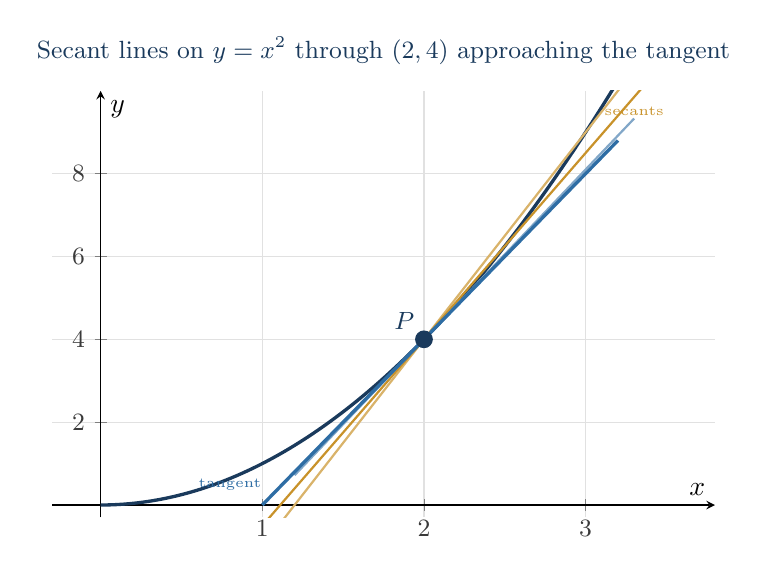
\begin{tikzpicture}
\begin{axis}[
  width=10cm, height=7cm,
  axis lines=center,
  xlabel={$x$}, ylabel={$y$},
  xmin=-0.3, xmax=3.8, ymin=-0.3, ymax=10,
  xtick={1,2,3}, ytick={2,4,6,8},
  tick label style={font=\small, color=DarkGrey},
  grid=major, grid style={DarkGrey!15},
  title={\small\color{NavyBlue}Secant lines on $y=x^2$ through $(2,4)$ approaching the tangent},
]
% Parabola
\addplot[NavyBlue, very thick, domain=0:3.5, samples=100] {x^2};
% Secant lines through (2,4) with different Q points
\addplot[Gold!70, thick, domain=0.5:3.5] {5*(x-2)+4};    % h=1: slope 5
\addplot[Gold, thick, domain=0.8:3.5]    {4.5*(x-2)+4};  % h=0.5: slope 4.5
\addplot[MidBlue!60, thick, domain=1.2:3.3] {4.1*(x-2)+4}; % h=0.1: slope 4.1
\addplot[MidBlue, very thick, domain=1.0:3.2] {4*(x-2)+4}; % tangent: slope 4
% Point P
\addplot[only marks, mark=*, mark size=3pt, color=NavyBlue] coordinates {(2,4)};
\node[color=NavyBlue, font=\small, above left] at (axis cs:2,4) {$P$};
\node[color=Gold, font=\tiny] at (axis cs:3.3,9.5) {secants};
\node[color=MidBlue, font=\tiny] at (axis cs:0.8,0.5) {tangent};
\end{axis}
\end{tikzpicture}
\end{center}

\begin{thought}
\textbf{What a tangent line actually is.}
In school geometry, a tangent to a circle is defined as a line that ``touches but does not cross'' the circle. This definition fails for most curves. A tangent to $y = x^3$ at the origin crosses the curve. A tangent to $y = \sin x$ at a zero also crosses it. The right definition --- the one calculus gives us --- is: the tangent line at a point is the \emph{limit of secant lines} as the second point approaches the first. This definition works for every smooth curve, agrees with the geometric intuition in simple cases, and breaks down precisely when the curve has a corner or a cusp. The failure of the limit at a corner is not a bug. It is correctly telling you that a corner has no well-defined direction.
\end{thought}

\subsection{Step 3: Different functions, different rates}

\begin{problem}
\label{prob:rates_general}
Use the limit process $\displaystyle\lim_{h \to 0} \frac{f(x+h) - f(x)}{h}$ to find the instantaneous rate of change of each function at the given point. Do each one algebraically --- do not guess.

\begin{enumerate}[label=(\alph*), topsep=2pt]
  \item $f(x) = x^2$ at $x = 3$
  \item $f(x) = x^3$ at $x = 1$
  \item $f(x) = x^2 + 3x$ at $x = 2$
  \item $f(x) = \dfrac{1}{x}$ at $x = 2$
  \item $f(x) = \sqrt{x}$ at $x = 4$ \quad \textit{(Hint: rationalise the numerator)}
\end{enumerate}

After completing all five, look at your results. Is there a pattern?
\end{problem}

\begin{problem}
\label{prob:pattern}
You should have noticed from Problem~\ref{prob:rates_general} that for $f(x) = x^n$, the rate of change at $x$ seems to follow a pattern.

\begin{enumerate}[label=(\alph*), topsep=2pt]
  \item State the pattern. Write it as a formula.
  \item Verify the pattern for $n = 4$ using the limit definition.
  \item Prove the pattern for general positive integer $n$. \textit{Hint: expand $(x+h)^n$ using the binomial theorem. What term survives after subtracting $x^n$ and dividing by $h$? What happens as $h \to 0$?}
  \item Does the pattern hold for $n = -1$? For $n = 1/2$? Check against your results in Problem~\ref{prob:rates_general}.
\end{enumerate}
\end{problem}

\begin{thought}
\textbf{The quarantine of 1665 and the general binomial theorem.}
When the Great Plague closed Cambridge University in 1665, 22-year-old Isaac Newton retreated to Woolsthorpe. In isolation, he generalized the binomial theorem to fractional and negative exponents, discovering that $(1+x)^\alpha = 1 + \alpha x + \frac{\alpha(\alpha-1)}{2!}x^2 + \cdots$ for any real $\alpha$. This allowed him to represent curves like $y = \sqrt{1-x^2} = (1-x^2)^{1/2}$ as infinite series and calculate their areas term-by-term. It was this algebraic breakthrough, rather than physics, that unlocked the calculus.
\end{thought}

\medskip
You have just discovered the \textbf{power rule} from first principles. The pattern $\frac{d}{dx}x^n = nx^{n-1}$ is one of the most-used facts in calculus, but its value lies not in memorising it --- it lies in knowing \emph{why} it is true, which you now do.


\subsection{Step 4: Rate of change as a new function}

\begin{problem}
\label{prob:deriv_as_func}
For $f(x) = x^2$, you found that the instantaneous rate of change at $x = 1$ is 2, at $x = 2$ is 4, at $x = 3$ is 6.
\begin{enumerate}[label=(\alph*), topsep=2pt]
  \item The instantaneous rate of change of $f$ at a general point $x$ is itself a function of $x$. Use the limit definition to find this function. Call it $f'(x)$.
  \item Plot $f(x) = x^2$ and $f'(x)$ on the same axes (use different colours). Describe their relationship.
  \item Where is $f(x) = x^2$ increasing? Decreasing? What does $f'(x)$ equal at those points?
  \item Now do the same for $f(x) = x^3$: find $f'(x)$ and plot both.
  \item For $h(t) = 20t - 5t^2$ from the opening puzzle: find $h'(t)$. At what time is $h'(t) = 0$? What does this mean physically?
\end{enumerate}
\end{problem}

\begin{thought}
\textbf{The derivative as a function.}
You have been computing the rate of change at specific points. But now you see that if you do this at every point simultaneously, you get a new function --- the \textbf{derivative}. The derivative $f'(x)$ tells you, at each $x$, how fast $f$ is changing. It is not just a number; it is a complete portrait of $f$'s behaviour. Where $f' > 0$, the function rises. Where $f' < 0$, it falls. Where $f' = 0$, it has a horizontal tangent --- a potential peak or trough.

This is why the derivative is so useful: it converts questions about the shape of a function (where is it increasing? where does it peak?) into questions about the sign and zeros of another function. The problem of understanding $f$ becomes the problem of reading $f'$.
\end{thought}

\begin{problem}
\label{prob:physical_meaning}
Each of the following gives a quantity as a function of time or position. In each case: find the rate of change function, and give a precise physical interpretation of what it measures.

\begin{enumerate}[label=(\alph*), topsep=2pt]
  \item $s(t) = 3t^2 + 2t$ (position in metres, $t$ in seconds). What is $s'(t)$? What is $s'(2)$?
  \item $V(r) = \frac{4}{3}\pi r^3$ (volume of a sphere of radius $r$). What is $V'(r)$? Recognise the answer.
  \item $A(s) = s^2$ (area of a square of side $s$). What is $A'(s)$? Interpret geometrically.
  \item $P(t) = 500 \cdot e^{0.1t}$ (population, $t$ in years). What is $P'(t)$? What fraction of the current population is the growth rate?
  \item $C(x) = 200 + 15x - 0.02x^2$ (cost in KES of producing $x$ units). What is $C'(x)$? This is called \emph{marginal cost} in economics. What does $C'(100) = 11$ mean in plain language?
\end{enumerate}
\end{problem}

% ============================================================
\section{Part 3 \texorpdfstring{---}{--} Discovery}
% ============================================================

\begin{discoverybox}
\textbf{What have we built?}

\textbf{First.} The instantaneous rate of change of a function $f$ at a point $x$ is the limit of average rates of change over shrinking intervals:
\[
  f'(x) \;=\; \lim_{h \to 0} \frac{f(x+h) - f(x)}{h}.
\]
This resolves the paradox of motion at an instant: instantaneous velocity is not a ratio of zero over zero. It is a \emph{limit} of ratios as the interval shrinks.

\textbf{Second.} Geometrically, $f'(x)$ is the slope of the tangent line to the graph of $f$ at the point $(x, f(x))$.

\textbf{Third.} The derivative is itself a function. Knowing $f'$ gives you a complete picture of where $f$ rises, falls, and levels off.

\textbf{Fourth.} The power rule $\frac{d}{dx}x^n = nx^{n-1}$ follows directly from the binomial theorem --- it is not magic, it is algebra.

\medskip
\textbf{Before reading on:} You found the derivative of $e^t$ in Journey~1 Module~5 (in the sense that $e^t$ is its own rate of change). Can you now state this precisely using the notation $f'(x) = \lim_{h\to 0}\frac{f(x+h)-f(x)}{h}$? Verify it using the series definition $e^x = \sum x^k/k!$.
\end{discoverybox}

% ============================================================
\section{Part 4 \texorpdfstring{---}{--} Naming the Idea}
% ============================================================

\begin{namebox}
\textbf{The derivative.}

Let $f : \mathbb{R} \to \mathbb{R}$. The \textbf{derivative} of $f$ at $x$ is
\[
  f'(x) \;=\; \lim_{h \to 0} \frac{f(x+h) - f(x)}{h},
\]
provided this limit exists. If it does, $f$ is called \textbf{differentiable} at $x$.

\medskip
\textbf{Notation.} Multiple notations are in use:
\[
  f'(x) \;=\; \frac{df}{dx} \;=\; \frac{d}{dx}f(x) \;=\; Df(x) \;=\; \dot{f}(x)\text{ (Newton's dot notation, used in physics)}.
\]
The notation $\frac{df}{dx}$ was introduced by \textbf{Leibniz}. The prime notation $f'$ was introduced by \textbf{Lagrange}. Newton used dots. All three are still in active use.

\medskip
\textbf{Power rule.} $\dfrac{d}{dx}x^n = nx^{n-1}$ for all $n$ (integers, rationals, reals --- though the proof for non-integers requires more work).

\medskip
\textbf{Geometric meaning.} $f'(x_0)$ is the slope of the tangent line to the graph of $f$ at the point $(x_0, f(x_0))$.

\medskip
\textbf{Physical meaning.} If $s(t)$ is position, then $s'(t)$ is velocity. If $v(t)$ is velocity, then $v'(t)$ is acceleration.
\end{namebox}

\begin{thought}
\textbf{Newton vs.\ Leibniz --- a bitter priority dispute.}
Isaac Newton developed his ``method of fluxions'' (his term for calculus) around 1666, but did not publish it until much later. Gottfried Leibniz developed calculus independently around 1675 and published in 1684 --- before Newton's first calculus publication. For decades afterwards, British and Continental mathematicians fought bitterly over who deserved credit. The dispute was partly genuine and partly nationalistic. Newton eventually wrote that Leibniz had ``stolen'' his ideas; Leibniz denied it. Modern historians generally believe both men made independent discoveries. The tragedy is that British mathematicians, out of loyalty to Newton, refused to use Leibniz's superior notation for over a century --- and fell a generation behind their Continental counterparts as a result. Notation is not neutral.
\end{thought}

% ============================================================
\section{Part 5 \texorpdfstring{---}{--} Deep Problems}
% ============================================================

\begin{deepproblem}[Differentiability vs.\ continuity]
\begin{enumerate}[label=(\alph*)]
  \item Prove that if $f$ is differentiable at $x_0$, then $f$ is continuous at $x_0$. \textit{Hint: write $f(x_0+h) - f(x_0) = \frac{f(x_0+h)-f(x_0)}{h} \cdot h$ and take $h \to 0$.}
  \item The converse is false. Show that $f(x) = |x|$ is continuous at $x = 0$ but not differentiable there. What goes wrong geometrically?
  \item The function $f(x) = x^{2/3}$ is continuous at $x = 0$. Is it differentiable? What does the tangent line look like at $x = 0$?
  \item \textit{(Surprising.)} In 1872, Karl Weierstrass exhibited a function that is continuous \emph{everywhere} but differentiable \emph{nowhere}:
  \[
    W(x) = \sum_{n=0}^{\infty} a^n \cos(b^n \pi x),
  \]
  for $0 < a < 1$, $b$ a positive odd integer, and $ab > 1 + 3\pi/2$. Describe intuitively why such a function is possible. What does this say about the relationship between continuity and smoothness?
\end{enumerate}
\end{deepproblem}

\begin{deepproblem}[The derivative of $e^x$ and $\sin x$]
\begin{enumerate}[label=(\alph*)]
  \item Using the series $e^x = \sum_{k=0}^{\infty} \frac{x^k}{k!}$, differentiate term by term to show $\frac{d}{dx}e^x = e^x$.
  \item The sine function has series $\sin x = x - \frac{x^3}{3!} + \frac{x^5}{5!} - \cdots$. Differentiate term by term. What do you get?
  \item Use the limit definition directly to verify $\frac{d}{dx}\sin x = \cos x$. You will need the limits $\lim_{h\to 0}\frac{\sin h}{h} = 1$ and $\lim_{h\to 0}\frac{\cos h - 1}{h} = 0$. Verify these two limits numerically.
  \item Differentiate $\cos x$ twice. What do you notice? Write a differential equation that $\cos x$ satisfies.
  \item What does the differential equation in (d) tell you about the physical systems that oscillate sinusoidally?
\end{enumerate}
\end{deepproblem}

\begin{deepproblem}[Higher-order derivatives and kinematics]
\begin{enumerate}[label=(\alph*)]
  \item If $f'(x)$ is itself differentiable, we can take its derivative: $f''(x) = (f')'(x)$. Compute $f''(x)$ for $f(x) = x^4 - 3x^2 + 2$.
  \item For position $s(t)$: $s'(t)$ is velocity, $s''(t)$ is acceleration. A particle has position $s(t) = t^3 - 6t^2 + 9t$. Find when it is at rest, when it moves forward, and when it is decelerating.
  \item The function $f(x) = e^x$ satisfies $f^{(n)}(x) = e^x$ for all $n$. Verify for $n = 1, 2, 3$. What is the $n$-th derivative of $\sin x$? Find the pattern and prove it.
  \item \textit{(Taylor series preview.)} If a function $f$ has derivatives of all orders at $x = 0$, we can write
  \[
    f(x) \approx f(0) + f'(0)x + \frac{f''(0)}{2!}x^2 + \frac{f'''(0)}{3!}x^3 + \cdots
  \]
  Apply this to $f(x) = e^x$ at $x = 0$. What do you get? Does it match the series you know?
\end{enumerate}
\end{deepproblem}

% ============================================================
\section{Part 6 \texorpdfstring{---}{--} Reflection}
% ============================================================

\begin{reflectionbox}
\textbf{Your reflection task.}

\begin{enumerate}
  \item \textbf{On the paradox.} At the start of this module, instantaneous speed seemed paradoxical --- $0/0$ is undefined. Write a paragraph explaining, in plain language, how the limit process resolves this. What is the key conceptual move that makes it work?

  \item \textbf{On Zeno.} Now that you have the limit definition of the derivative, revisit Zeno's arrow paradox. Is the paradox resolved? Or has it merely been reformulated? Write two sentences: one arguing that calculus solves Zeno, and one arguing that it does not.

  \item \textbf{On notation.} You learned three notations for the derivative: $f'(x)$, $\frac{df}{dx}$, and $\dot{f}$. Which do you find most natural? The note on the Newton--Leibniz dispute suggests that notation has real consequences. Can you think of a case in which the notation you use for something shapes how you think about it?

  \item \textbf{Looking ahead.} Module~2 will derive rules that let you differentiate any combination of functions without returning to the limit definition each time. The chain rule, product rule, and quotient rule. Before you are taught them: if $f$ and $g$ are both differentiable, how do you think $(f \cdot g)'$ and $(f \circ g)'$ should behave? Write a guess for each.
\end{enumerate}
\end{reflectionbox}

\medskip
\noindent\textbf{Looking ahead.}
Module~2 derives the differentiation rules --- product, quotient, and chain --- that make it practical to differentiate compound expressions without returning to the limit definition each time. These rules are not arbitrary tricks. Each one follows from the limit definition by a single careful algebraic argument, and each one has a geometric or physical interpretation that is worth understanding.

Module~3 will then ask the inverse question: if $f'(x)$ is known, what can we say about $f(x)$ itself? The answer is the integral --- and the remarkable connection between differentiation and integration is the deepest theorem in all of calculus.

\vspace{1.4cm}
\begin{center}
{\color{MidBlue}\rule{0.5\linewidth}{0.8pt}}\\[6pt]
{\small\color{DarkGrey}\textit{End of Journey 2, Module 1 --- Motion and Rate}}\\[4pt]
{\small\color{DarkGrey}Continue to: \textbf{Module 2 --- The Derivative}}\\[6pt]
{\color{MidBlue}\rule{0.5\linewidth}{0.8pt}}
\end{center}

\end{document}